% Options for packages loaded elsewhere
\PassOptionsToPackage{unicode}{hyperref}
\PassOptionsToPackage{hyphens}{url}
\PassOptionsToPackage{dvipsnames,svgnames,x11names}{xcolor}
\documentclass[
  10pt,
  fontset=fandol]{ctexart}
\usepackage{xcolor}
\usepackage[margin=16mm]{geometry}
\usepackage{amsmath,amssymb}
\setcounter{secnumdepth}{-\maxdimen} % remove section numbering
\usepackage{iftex}
\ifPDFTeX
  \usepackage[T1]{fontenc}
  \usepackage[utf8]{inputenc}
  \usepackage{textcomp} % provide euro and other symbols
\else % if luatex or xetex
  \usepackage{unicode-math} % this also loads fontspec
  \defaultfontfeatures{Scale=MatchLowercase}
  \defaultfontfeatures[\rmfamily]{Ligatures=TeX,Scale=1}
\fi
\usepackage{lmodern}
\ifPDFTeX\else
  % xetex/luatex font selection
\fi
% Use upquote if available, for straight quotes in verbatim environments
\IfFileExists{upquote.sty}{\usepackage{upquote}}{}
\IfFileExists{microtype.sty}{% use microtype if available
  \usepackage[]{microtype}
  \UseMicrotypeSet[protrusion]{basicmath} % disable protrusion for tt fonts
}{}
\makeatletter
\@ifundefined{KOMAClassName}{% if non-KOMA class
  \IfFileExists{parskip.sty}{%
    \usepackage{parskip}
  }{% else
    \setlength{\parindent}{0pt}
    \setlength{\parskip}{6pt plus 2pt minus 1pt}}
}{% if KOMA class
  \KOMAoptions{parskip=half}}
\makeatother
\usepackage{longtable,booktabs,array}
\newcounter{none} % for unnumbered tables
\usepackage{calc} % for calculating minipage widths
% Correct order of tables after \paragraph or \subparagraph
\usepackage{etoolbox}
\makeatletter
\patchcmd\longtable{\par}{\if@noskipsec\mbox{}\fi\par}{}{}
\makeatother
% Allow footnotes in longtable head/foot
\IfFileExists{footnotehyper.sty}{\usepackage{footnotehyper}}{\usepackage{footnote}}
\makesavenoteenv{longtable}
\usepackage{graphicx}
\makeatletter
\newsavebox\pandoc@box
\newcommand*\pandocbounded[1]{% scales image to fit in text height/width
  \sbox\pandoc@box{#1}%
  \Gscale@div\@tempa{\textheight}{\dimexpr\ht\pandoc@box+\dp\pandoc@box\relax}%
  \Gscale@div\@tempb{\linewidth}{\wd\pandoc@box}%
  \ifdim\@tempb\p@<\@tempa\p@\let\@tempa\@tempb\fi% select the smaller of both
  \ifdim\@tempa\p@<\p@\scalebox{\@tempa}{\usebox\pandoc@box}%
  \else\usebox{\pandoc@box}%
  \fi%
}
% Set default figure placement to htbp
\def\fps@figure{htbp}
\makeatother
\setlength{\emergencystretch}{3em} % prevent overfull lines
\providecommand{\tightlist}{%
  \setlength{\itemsep}{0pt}\setlength{\parskip}{0pt}}
\usepackage{amsmath,amssymb,mathtools,needspace}
\xeCJKDeclareCharClass{CJK}{"2032,"0400->"04FF,"2160->"216B,"2460->"2473,"25A0,"25C7,"25CB,"25CF}
\IfFontExistsTF{Arial Unicode MS}{\xeCJKsetup{AutoFallBack=true}\setCJKfallbackfamilyfont{\CJKrmdefault}{Arial Unicode MS}}{}
\setcounter{secnumdepth}{0}
\setlength{\emergencystretch}{2em}
\allowdisplaybreaks
\usepackage{bookmark}
\IfFileExists{xurl.sty}{\usepackage{xurl}}{} % add URL line breaks if available
\urlstyle{same}
\hypersetup{
  pdftitle={``结绳记数''的快速算法},
  colorlinks=true,
  linkcolor={Maroon},
  filecolor={Maroon},
  citecolor={Blue},
  urlcolor={Blue},
  pdfcreator={LaTeX via pandoc}}

\title{``结绳记数''的快速算法}
\author{}
\date{}

\begin{document}
\maketitle

\subsubsection{13.5.1 ``结绳记数''的快速算法}\label{ux7ed3ux7ef3ux8bb0ux6570ux7684ux5febux901fux7b97ux6cd5}

考古发现，上古没有文字，中华先民靠在绳索上打结的办法来记录数字，这就是所谓的``结绳记数''。

结绳记数有许多优点：绳结容易制作，造价低廉；打结方法简单，无需附加工具；绳结可随意变形，保管携带都很方便。绳结是个理想的``数字存储器''。

绳结可以用来记数，这是古人早就认识到的。问题在于，如果一条绳结上存有大量结点，逐个累加不但枯燥乏味，而且效率低下，那么该怎样快速地求出结点总数呢？熟知``刚柔相推，变在其中''（《周易·系辞》）的中华先贤自然早就知道，``软硬兼施''的绳结有一种快速计数方法。

设绳结上的结点是等距排列的。试将它对折为两半，并令其首尾两个结点对齐

\href{../../source-images/pdf-315.jpeg}{原页图像}

（见图 13.1）。设用阴阳二分点来刻画结点数是偶数还是奇数：若结点数为偶数，则二分点是个虚的结点，记作``●''；若结点数为奇数，则二分点是个实的结点，记作``○''。这种\textbf{二分手续}取得了``大事化小''的效果。

对二分后的子段又可继续施行上述二分手续，从而产生一个新的二分点 ● 或 ○。这样反复做下去，直到子段上仅含一个结点为止。最终留下的一个结点自然视为二分点 ○。这样，二分过程最终实现了``小事化了''的目标。

绳结的这种二分演化过程如图 13.1 所示。

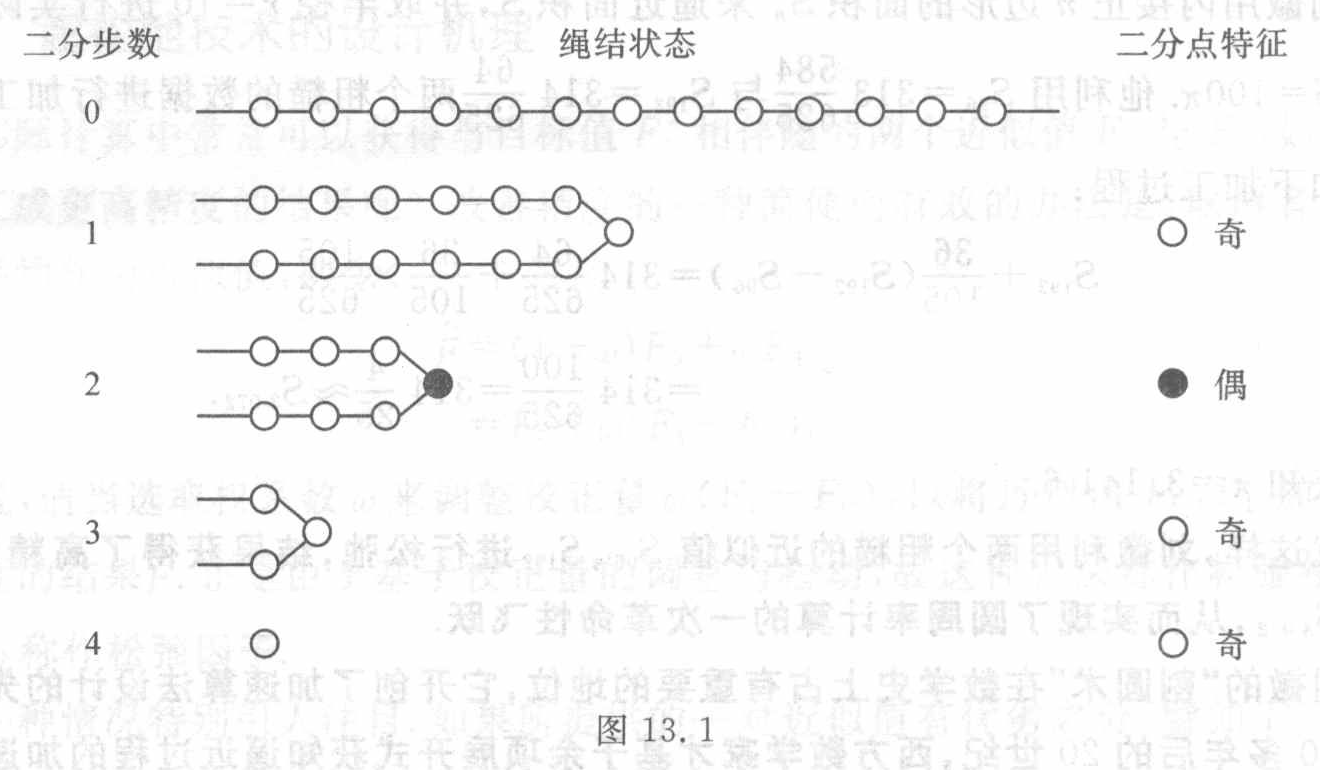
\includegraphics[width=0.85\linewidth,height=\textheight,keepaspectratio,alt={图 13.1（原图）}]{../assets/ch13/fig-13-1.png}

图 13.1

\begin{quote}
图意及标签转录（据原图）：原图三列为``二分步数''\,``绳结状态''\,``二分点特征''。第 0 步为包含 13 个空心结点的直绳；第 1 步将绳对折，两侧各 6 个空心结点，对折处为一个空心结点；第 2 步的两侧各 3 个空心结点，对折处标为实心圆；第 3 步的两侧各 1 个空心结点，对折处为一个空心结点；第 4 步仅余一个空心结点。二分点特征栏的全部标记为：
\end{quote}

{\def\LTcaptype{none} % do not increment counter
\begin{longtable}[]{@{}ll@{}}
\toprule\noalign{}
二分步数 & 二分点特征 \\
\midrule\noalign{}
\endhead
\bottomrule\noalign{}
\endlastfoot
0 & （原图留空） \\
1 & ○ 奇 \\
2 & ● 偶 \\
3 & ○ 奇 \\
4 & ○ 奇 \\
\end{longtable}
}

在上述二分演化过程中，逐步生成了一个二分点的序列。设将先后生成的二分点从右往左顺序排列，即可生成一个有方向、有层次的虚拟绳结（见图 13.2）。这个虚拟绳结同原先的绳结（见图 13.1）的含义一致，但信息量被大大地压缩了。

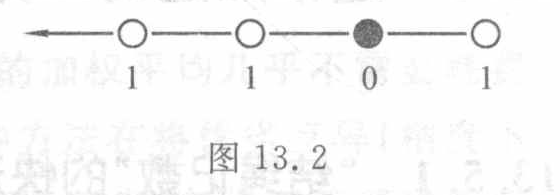
\includegraphics[width=0.42\linewidth,height=\textheight,keepaspectratio,alt={图 13.2（原图）}]{../assets/ch13/fig-13-2.png}

图 13.2

\begin{quote}
图意及标签转录（据原图）：箭头指向左方；沿水平绳从左到右的四个结点依次为 ○、○、●、○，其下数字依次为 \(1,1,0,1\)。
\end{quote}

设原先的绳结数为 \(N\)，则二分过程的信息压缩比

\[
\frac{N}{\log_2N}\longrightarrow+\infty.
\]

一个出人意料的结论是，如果将虚拟绳结的虚实结点 ● 与 ○ 分别赋值 0 与 1，即可得到所求绳结数的二进制数 \((1101)_2=13\)。

\textbf{摆弄绳结可以孕育出二进制，这是一个奇妙的事实，这一事实表现了中华古算的博大精深。}

\end{document}
